
\section{Teori}

    \textbf{Motivasjon og sammenheng:} For å forstå hvorfor det er en grense på 100 meter for Ethernet-kabler, og hvordan signaler dempes og forvrenges i slike kabler, må vi bruke telegraflikningen. Denne beskriver hvordan elektriske signaler forplanter seg i transmisjonslinjer, og gir oss verktøyene til å analysere tap, dispersjon.

\subsection{Fourierrekker}

Mange signaler kan brytes ned i sine frekvenskomponenter ved hjelp av Fourier-analyse. Dette er spesielt nyttig i signalbehandling og for å forstå hvordan ulike frekvenser påvirkes av transmisjonslinjen. Vi bruker Fourier-rekker for endelige intervaller (Dirichlet/Neumann). Ethernet-signaler kan sees på som en sekvens av pulser (bitstrøm), som i praksis kan betraktes som et periodisk pulstog. Dette gjør at Fourierrekker er et naturlig verktøy for å analysere slike signaler i frekvensdomenet, siden pulstoget kan uttrykkes som en sum av sinus- og cosinuskomponenter.\\[1em]
En periodisk funksjon $f(t)$ med periode $T$ kan uttrykkes som en Fourier-rekke:
\begin{equation}
f(t) = a_0 + \sum_{n=1}^{\infty} \left( a_n \cos\left(\frac{2\pi n t}{T}\right) + b_n \sin\left(\frac{2\pi n t}{T}\right) \right)
\end{equation}
med koeffisienter gitt ved:
\begin{align*}
a_0 &= \frac{1}{T} \int_{0}^{T} f(t) \, dt \\
a_n &= \frac{2}{T} \int_{0}^{T} f(t) \cos\left(\frac{2\pi n t}{T}\right) dt \\
b_n &= \frac{2}{T} \int_{0}^{T} f(t) \sin\left(\frac{2\pi n t}{T}\right) dt
\end{align*}
I Komplekse form:
\begin{equation}
f(t) = \sum_{n=-\infty}^{\infty} c_n e^{i \frac{2\pi n t}{T}}, \quad \text{der} \quad c_n = \frac{1}{T} \int_{0}^{T} f(t) e^{-i \frac{2\pi n t}{T}} dt
\end{equation}
I dette prosjektet vil vi bruke Fourier-analyse for å dekomponere Ethernet-signaler i sine frekvenskomponenter, slik at vi kan studere hvordan hver komponent påvirkes av transmisjonslinjens egenskaper.
Ved å gjennomføre målinger for forskjellige kabellengder, kan vi sammenligne de målte dataene med de teoretiske prediksjonene basert på Fourier-analyse og telegraflikningen.
Vi får da overføringsfunksjonen for kabelen.
\begin{equation}
    H(f) = \frac{V_{out}(f)}{V_{in}(f)}
\end{equation}
Som beskriver hvordan signalet endres i frekvensdomenet når det passerer gjennom kabelen.
Denne analysen hjelper oss å forstå hvordan ulike frekvenskomponenter dempes og forvrenges, noe som er avgjørende for å forklare begrensningen på kabelens lengde.
Setter vi inn overførsingsfunksjonen i komplekse Fourier-rekken, kan vi modellere hvordan hele signalet endres når det går gjennom kabelen.
\begin{equation}
    f_{out}(t) = \sum_{n=-\infty}^{\infty} H\left(\frac{n}{T}\right) c_n e^{i \frac{2\pi n t}{T}}
\end{equation}
\subsection{Telegraflikningen og transmisjonslinjer}
En transmisjonslinje kan beskrives ved fire per-enhet-lengde parametre:
\begin{itemize}
    \item $R$ \, [$\Omega$/m] \,-- motstand (ledertap),
    \item $L$ \, [H/m] \,-- induktans (magnetisk lagring),
    \item $C$ \, [F/m] \,-- kapasitans (elektrisk lagring),
    \item $G$ \, [S/m] \,-- ledningsevne (lekkasjetap).
\end{itemize}
Ved å kombinere Kirchhoffs lover med disse parameterne utledes telegrafligningen, som beskriver spenning og strøm som funksjon av både posisjon og tid langs kabelen. For spenningen $u(x,t)$ kan den skrives på formen:
\begin{equation}
    u_{tt} + (RG + LC)u_t + RG\,u = c^2 u_{xx}, \qquad c = \frac{1}{\sqrt{LC}} ,
\end{equation}
der $u(x,t)$ er spenningen langs kabelen og $c$ er utbredelseshastigheten i kabelen.  
Denne ligningen viser at et signal ikke bare forplanter seg med en hastighet bestemt av $L$ og $C$, men også blir dempet og forvrengt på grunn av $R$ og $G$. Resultatet er at høyfrekvente komponenter i signalet svekkes og spres mer enn lave frekvenser, noe som over tid fører til \emph{demping og dispersjon}.  
Ethernet-signaler består ikke av rene sinusbølger, men av pulser med et bredt spekter av frekvenser. Med Fourier-analyse kan signalet uttrykkes som en sum av slike frekvenskomponenter, og telegrafligningen gir oss verktøy til å studere hvordan hver enkelt komponent påvirkes. Dermed kan vi forklare hvorfor en grense på omtrent 100 meter er praktisk: etter denne lengden er tapet og forvrengningen så store at signalet ikke lenger kan tolkes pålitelig av mottakeren.


\subsubsection{R - Resistans}
Resistans per lengde $[\Omega/\mathrm{m}]$ er den ohmske motstanden i lederen. Den skyldes av materialets resistivitet og ledertverrsnitt, og øker med temperatur. Motstanden øker dempingen og rekkevidden til signalet. I telegrafligningen bidrar R direkte til tidsdemping av både strøm og spenning.

\subsubsection{L - Induktans}
Induktansen per lengde $[\mathrm{L}/\mathrm{m}]$ er magnetisk lagring av energi rundt lederen når strømmen endres, per meter kabel. Sammen med kapasitans vil denne bestemme farten på signalet i kabelen. I linjemodellen er induktans i seriekobling.

\subsubsection{C - Kapasitans}
Kapasitans per lengde $[\mathrm{C}/\mathrm{m}]$ er elektrisk lagring av energi i feltet mellom leder og referanse, per meter. Sammen med induktans har kapasitans påvirkning på fart. I linjemodellen er dette en gren til jord, den trekker ladning når spenningen endres.

\subsubsection{G - Ledningsevne}
Ledningsevnen per meter $[\mathrm{G}/\mathrm{m}]$ beskriver det dielektriske taper gjennom isolasjonen til jord, per meter. Det påvirker signalet i form av å øke dempingen fordi energi vil lekke i dielektrikumet. Høy fuktighet eller dårlig isolasjon vil svekke ledningsevnen. Ledningsevnen opererer i parallelt med kapasitansen i linjemodellen.









\subsubsection{Utledning av telegraflikningen}
Telegraflikningen kan utledes ved å analysere en liten del av transmisjonslinjen, som vist i figuren nedenfor. Vi betrakter et segment av linjen med lengde $\Delta x$, og bruker Kirchhoffs spennings- og strømlov for å sette opp differensialligninger for spenning og strøm.
\begin{figure}[h]
    \centering
    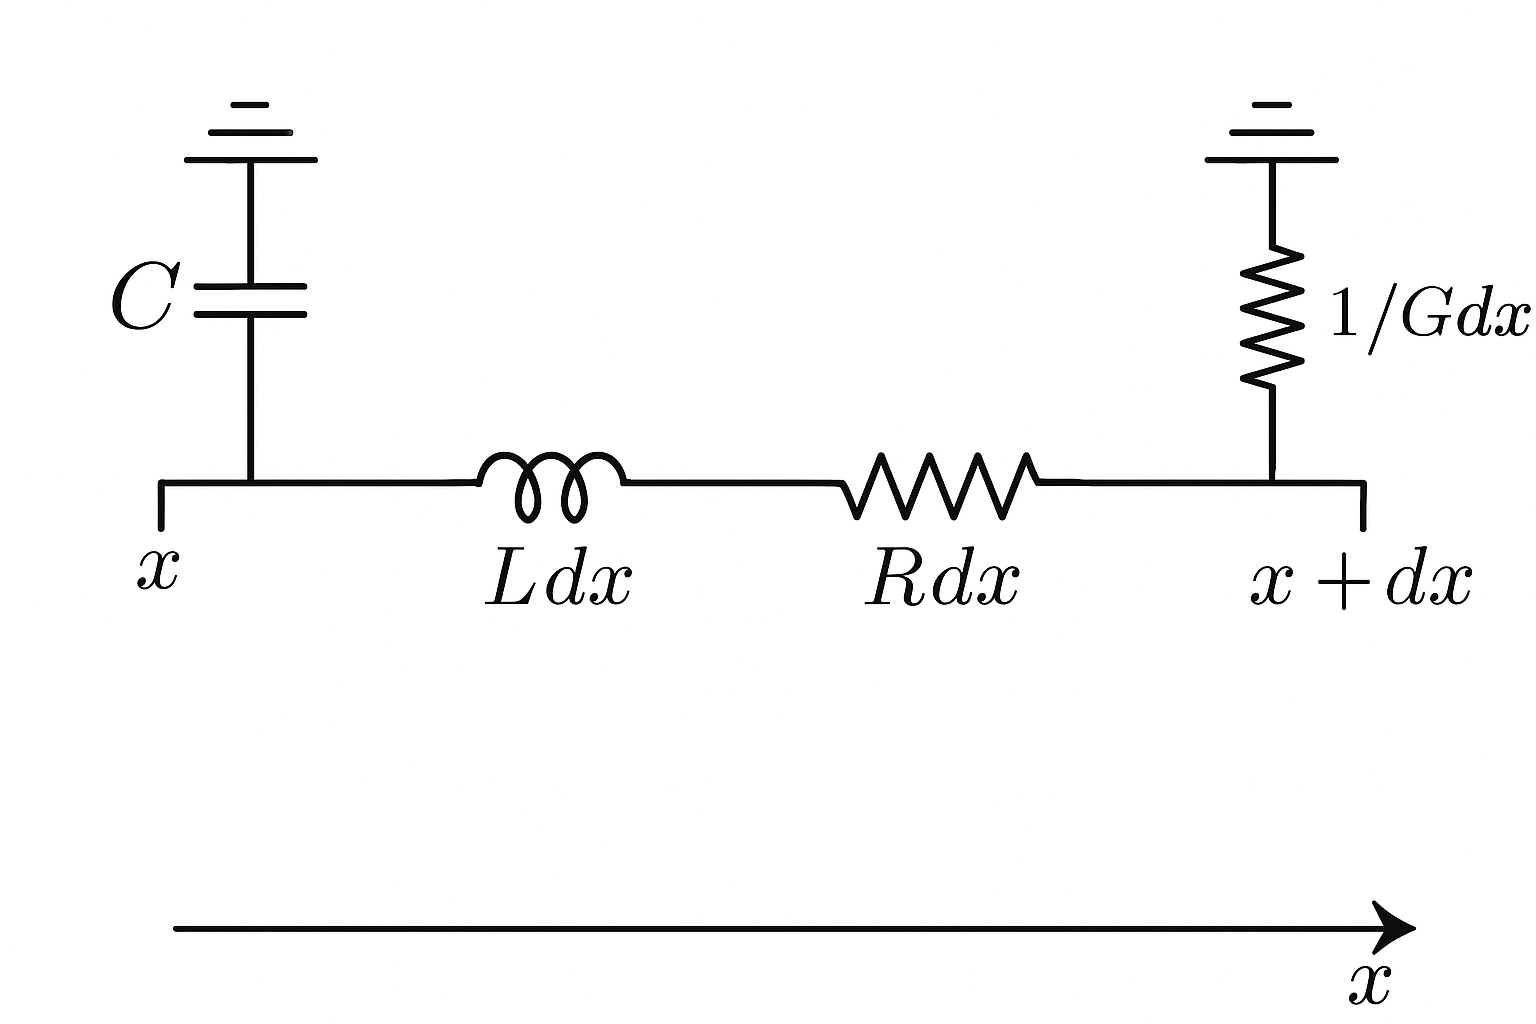
\includegraphics[width=0.6\textwidth]{Media/telegraflinje.png}
    \caption{Elementær segment av en transmisjonslinje med per-enhet-lengde parametere.}
    \label{fig:transmission_line_segment}   
\end{figure}
Ved å anvende Kirchhoffs spenningslov på segmentet får vi:
\begin{equation}
    u(x,t) - u(x+\Delta x,t) = R \Delta x \cdot i(x,t) + L \Delta x \cdot \frac{\partial i(x,t)}{\partial t} .
\end{equation}
Ved å la $\Delta x \to 0$ får vi den første differensialligningen:
\begin{equation}
    \frac{\partial u(x,t)}{\partial x} = -R i(x,t) - L \frac{\partial i(x,t)}{\partial t} . 
\end{equation}
Tilsvarende, ved å bruke Kirchhoffs strømlov, får vi:
\begin{equation}
    i(x,t) - i(x+\Delta x,t) = -G \Delta x \cdot u(x,t) - C \Delta x \cdot \frac{\partial u(x,t)}{\partial t} .
\end{equation}
Igjen, ved å la $\Delta x \to 0$ får vi den andre differensialligningen:
\begin{equation}
    \frac{\partial i(x,t)}{\partial x} = -G u(x,t) - C \frac{\partial u(x,t)}{\partial t} .
\end{equation}
Ved å derivere den første ligningen med hensyn på $x$ og den andre med hensyn på $t$, og deretter eliminere $i(x,t)$, får vi telegraflikningen for spenningen:
\begin{equation}
    u_{tt} + (RG + LC)u_t + RG\,u = c^2 u_{xx}, \qquad c = \frac{1}{\sqrt{LC}} .
\end{equation}
Dette kan vi skrive som:
\begin{equation}
    u_{tt} + (\alpha + \beta)u_t + \alpha \beta u = c^2 u_{xx}, \qquad c = \frac{1}{\sqrt{LC}} ,
\end{equation}
der vi har definert:
\begin{equation}
    \alpha = \frac{R}{L}, \qquad \beta = \frac{G}{C} .
\end{equation}
Dette er en dampet bølgeligning som beskriver hvordan spenningen forplanter seg langs transmisjonslinjen, med demping og forvrengning bestemt av parametrene $R$, $L$, $C$, og $G$.



\paragraph{Løsning av randverdiproblemet og valg av koeffisienter}

Vi løser nå randverdiproblemet
\begin{align}
  &u_{tt}+(\alpha+\beta)u_t+\alpha\beta\,u = c^2 u_{xx}, \tag{1}\\
  &u(0,t)=0, \tag{2}\\
  &u(\ell,t)=0, \tag{3}\\
  &u(x,0)=\delta(x-a), \tag{4}\\
  &u_t(x,0)=0, \tag{5}
\end{align}
for alle $t>0$ og $0<x<\ell$. Dette modellerer en telegraflinje av lengde $\ell$ med spenningsnull i begge ender, og en ideell startimpuls lokalisert i $x=a$ som i utgangspunktet er stasjonær.

\paragraph{Separasjon av variabler.}
Vi prøver $u(x,t)=X(x)T(t)$. Setter dette inn i (1):
\[
XT'' + (\alpha+\beta)XT' + \alpha\beta XT
\;=\; c^2 X''T.
\]
Vi deler på $XT$ og får
\[
\frac{1}{c^2}\!\left(\frac{T''}{T} + (\alpha+\beta)\frac{T'}{T} + \alpha\beta\right) \;=\; \frac{X''}{X} \;=\; \sigma,
\]
der $\sigma$ er en separasjonskonstant. Denne er konstant siden venstresiden avhenger bare av $t$ og høyresiden bare av $x$, begge sider må være konstant.

\paragraph{Romdel og randbetingelser.}
Randbetingelsene (2)--(3) krever $X(0)=X(\ell)=0$. Romlikningen er
\[
X'' - \sigma X = 0.
\]
Ikke-trivielle løsninger som tilfredsstiller faste ender oppnås ved

\[
\sigma = -\Big(\frac{n\pi}{\ell}\Big)^2, \qquad
X_n(x)=\sin\!\Big(\frac{n\pi x}{\ell}\Big), \qquad n=1,2,\dots
\]
(her er $X_n''=-(n\pi/\ell)^2 X_n$ og $X_n(0)=X_n(\ell)=0$).

\paragraph{Tidsdel per modus.}
For gitt $n$ blir tidslikningen
\[
T'' + (\alpha+\beta)T' + \big(\alpha\beta - \sigma c^2\big)\,T \;=\; 0
\;\;\Longleftrightarrow\;\;
T'' + (\alpha+\beta)T' + \Big(\alpha\beta + c^2\Big(\frac{n\pi}{\ell}\Big)^2\Big)T = 0.
\]
Det karakteristiske polynomet gir røtter
\[
r_i = \frac{1}{2}\!\left(-\alpha-\beta \pm \sqrt{(\alpha+\beta)^2 - 4\alpha\beta + 4c^2\Big(\frac{n\pi}{\ell}\Big)^2}\right).
\]
Sett
\[
d=\frac{\alpha+\beta}{2}, \qquad
\omega_n = \sqrt{\,c^2\Big(\frac{n\pi}{\ell}\Big)^2 - \frac{1}{4}(\alpha-\beta)^2\,}.
\]
Da er $r_i=-d\pm i\omega_n$, og en praktisk realform av løsningen er
\[
T_n(t)=A_n e^{-dt}\cos(\omega_n t - \phi_n),
\]
med fri amplitude $A_n$ og fase $\phi_n$ (bestemmes av (4)--(5)).




\paragraph{Seriesløsning og løsning av initialverdier}

Vi har fra separasjon av variabler at løsningene med faste ender $x=0$ og $x=\ell$ kan bygges som en superposisjon av romlige egenfunksjoner
\[
X_n(x)=\sin\!\Big(\frac{n\pi x}{\ell}\Big),\qquad n=1,2,\dots
\]
multiplisert med tilhørende tidsfaktorer. I det underdempede tilfellet (der \(\omega_n>0\), se definisjon nedenfor) kan tidsdelen skrives på realform med demping og fase. Summen over alle moduser blir
\begin{equation}\label{eq:series-solution}
u(x,t)=\sum_{n=1}^{\infty} A_n\,e^{-dt}\cos\!\big(\omega_n t-\phi_n\big)\,
\sin\!\Big(\frac{n\pi x}{\ell}\Big),
\end{equation}
der parameterne er
\[
d=\frac{\alpha+\beta}{2},\qquad
\omega_n=\sqrt{\,c^2\Big(\frac{n\pi}{\ell}\Big)^2-\frac{1}{4}(\alpha-\beta)^2\,}.
\]
Uttrykket \eqref{eq:series-solution} tilfredsstiller allerede PDE-en og randbetingelsene i endepunktene. Det som gjenstår er å bestemme amplituder $A_n$ og faser $\phi_n$ slik at startbetingelsene oppfylles på $t=0$.

\paragraph{Trinn 1: Bruk av $u_t(x,0)=0$.}
Vi deriverer \eqref{eq:series-solution} i tid og setter $t=0$:
\[
u_t(x,0)=\sum_{n=1}^{\infty} A_n\Big[-d\cos\phi_n+\omega_n\sin\phi_n\Big]\,
\sin\!\Big(\frac{n\pi x}{\ell}\Big).
\]
Siden \(\{\sin(n\pi x/\ell)\}_{n\ge 1}\) er ortogonal og fullstendig på \((0,\ell)\) med faste ender, må hver Fourier-koeffisient være null for at $u_t(x,0)$ skal være identisk null. Dermed får vi, for hvert $n$,
\begin{equation}\label{eq:phase-eq}
-d\cos\phi_n+\omega_n\sin\phi_n=0
\quad\Longrightarrow\quad
\phi_n=\arctan\!\Big(\frac{d}{\omega_n}\Big).
\end{equation}
Denne relasjonen sier at fasen bestemmes entydig av forholdet mellom dempningsraten \(d\) og egenfrekvensen \(\omega_n\): jo sterkere demping i forhold til svingning, desto større faseforskyvning i tidsfaktoren.

\paragraph{Trinn 2: Bruk av $u(x,0)=\delta(x-a)$.}
Setter vi $t=0$ i \eqref{eq:series-solution} og benytter \(\cos(-\phi_n)=\cos\phi_n\), får vi
\[
u(x,0)=\sum_{n=1}^{\infty} A_n\cos\phi_n\,\sin\!\Big(\frac{n\pi x}{\ell}\Big).
\]
Startprofilen er en ideell spiss plassert i \(x=a\), dvs.\ \(\delta(x-a)\). Dens sinusutvikling på \((0,\ell)\) er
\[
\delta(x-a)=\sum_{n=1}^{\infty}\Big(\frac{2}{\ell}\sin\!\frac{n\pi a}{\ell}\Big)\,
\sin\!\Big(\frac{n\pi x}{\ell}\Big),
\]
som følger ved å projisere mot \(\sin(n\pi x/\ell)\) og bruke
\[
\int_0^\ell \delta(x-a)f(x)\,dx=f(a),\qquad
\int_0^\ell \sin^2\!\Big(\frac{n\pi x}{\ell}\Big)\,dx=\frac{\ell}{2}.
\]
Identifikasjon av koeffisientene gir derfor
\begin{equation}\label{eq:Acosphi}
A_n\cos\phi_n=\frac{2}{\ell}\,\sin\!\Big(\frac{n\pi a}{\ell}\Big).
\end{equation}

\paragraph{Amplituder og faser eksplisitt.}
Fra \eqref{eq:phase-eq} har vi
\[
\cos\phi_n=\frac{\omega_n}{\sqrt{\omega_n^2+d^2}},\qquad
\sin\phi_n=\frac{d}{\sqrt{\omega_n^2+d^2}}.
\]
Setter vi dette inn i \eqref{eq:Acosphi}, fås en praktisk eksplisitt amplitude
\begin{equation}\label{eq:An-explicit}
A_n=\frac{2}{\ell}\,\frac{\sqrt{\omega_n^2+d^2}}{\omega_n}\,
\sin\!\Big(\frac{n\pi a}{\ell}\Big),
\qquad
\phi_n=\arctan\!\Big(\frac{d}{\omega_n}\Big).
\end{equation}
Alternativt, og ofte penere i kompakt form, skriver vi amplituden direkte i samme stil som i oppsettet over:
\begin{equation}\label{eq:An-cosphi}
A_n=\frac{2}{\ell}\,\frac{1}{\cos\phi_n}\,
\sin\!\Big(\frac{n\pi a}{\ell}\Big),
\qquad
\phi_n \text{ gitt av \eqref{eq:phase-eq}.}
\end{equation}

\paragraph{Endelig løsning og tolkning.}
Setter vi \eqref{eq:An-cosphi} og \eqref{eq:phase-eq} inn i \eqref{eq:series-solution}, får vi den endelige seriesummen
\begin{equation}\label{eq:final-solution}
u(x,t)=\sum_{n=1}^{\infty} A_n\,e^{-dt}\cos\!\big(\omega_n t-\phi_n\big)\,
\sin\!\Big(\frac{n\pi x}{\ell}\Big),
\quad
A_n=\frac{2}{\ell}\,\frac{1}{\cos\phi_n}\sin\!\Big(\frac{n\pi a}{\ell}\Big),
\quad
\phi_n=\arctan\!\Big(\frac{d}{\omega_n}\Big).
\end{equation}
Hvert romlig modus \(\sin(n\pi x/\ell)\) oscillerer i tid med vinkelhastighet \(\omega_n\) og dempes med rate \(d=(\alpha+\beta)/2\). Fasene \(\phi_n\) er valgt slik at hastighetsbetingelsen \(u_t(x,0)=0\) oppfylles koeffisientvis. Startimpulsen i \(x=a\) fordeler seg på alle moduser gjennom vektene \(\sin(n\pi a/\ell)\); moduser med et nullpunkt i \(x=a\) (\(\sin(n\pi a/\ell)=0\)) blir ikke eksitert.

\medskip
\noindent
\emph{Merknad om dempningsregimer.} Når \(\omega_n>0\) (underdempet) har vi formen \(\mathrm{e}^{-dt}\cos(\omega_n t-\phi_n)\). I grensefallet \(\omega_n=0\) (kritisk demping) og for \(\omega_n^2<0\) (overdempet) erstattes denne av de tilsvarende reelle eksponentialformene for tidsløsningen. Fremgangsmåten for å bestemme koeffisienter via \eqref{eq:phase-eq}–\eqref{eq:Acosphi} er ellers uendret.

\subsubsection{Idealpuls}


I modellen brukes \(u(x,0)=\delta(x-a)\) som en idealpuls med svært kort varighet. Den inneholder rikelig med høye frekvenser, altså nettopp de komponentene som bestemmer kantskarphet i digitale signaler. I et praktisk oppsett med funksjonsgenerator og oscilloskop blir to forhold avgjørende for tolkningen: (i) generatorens endelige båndbredde (og tilsvarende stigetid) gjør at innsignalet ikke er ideelt skarpt, og (ii) oscilloskopets båndbredde og tidsoppløsning begrenser hva som faktisk registreres av raske endringer. 

Disse rammene er viktige fordi de påvirker hvordan kabelens ekstra demping og utglatting av de høyfrekvente komponentene fremtrer i målekurvene. Når de høyeste frekvensene svekkes med lengde, øker stigetid og hale, og bitene blir mindre adskilt. Dette er samme mekanisme som gjør at en kabel på omkring 100\,m nærmer seg grensen for pålitelig deteksjon ved gitt symbolhastighet: ikke bare faller nivået, men kantinformasjonen utvannes.





\subsection{Metoder og praktisk relevans}

(a) \textit{Fourierrekker:} Analytisk på $[0,L]$ (m/Dirichlet) for å vise $\alpha=\beta$-tilfellet.\\
\dots
\clearpage
\subsection{Dispersjon}

Dispersjon betyr at ulike frekvenskomponenter i en bølge forplanter seg med forskjellig hastighet. 
I telegrafligningen oppstår dette fordi bølgefarten $v_n$ avhenger av frekvensen og parameterne 
$R$, $L$, $C$ og $G$. 

Konsekvensen er at et signal som består av mange frekvenser (for eksempel en skarp puls) gradvis 
forvrenges når det forplanter seg. Dette er en sentral utfordring i signaloverføring: skarpe signaler 
blir bredere og mister form over tid. 
\dots

\subsection{Oppsummering og kobling til prosjektet}

Teorien over forklarer hvorfor signaler i lange kabler dempes og forvrenges, og gir oss verktøyene til å analysere dette både analytisk og numerisk. Dette er avgjørende for å forstå hvorfor det er en 100 m-grense for Ethernet-kabler. I det videre arbeidet skal vi først gjennomføre praktiske målinger, og deretter \textcolor{red}{numeriske simuleringer} (kanskje), slik at begge kan sammenlignes med de teoretiske resultatene for å se hvordan modellen stemmer med virkeligheten.
